\clearpage

\begin{flushright}
  \fechaclase{24 de septiembre de 2026}
\end{flushright}

\paragraph{\tituloejemplo{Ejemplo}}
Verifique el funcionamiento del controlador para
\[
  \dot{X}_1=X_2
\]
\[
  \dot{X}_2=\operatorname{sen}(X_1X_2)+\cos(X_1+X_2)+u
\]
\[
  y=X_1
\]

\paragraph{Resolución}

El controlador se implementa dentro de un bloque \texttt{MATLAB Function}:

\begin{MatlabCode}
function [du, sigma]= controlador(x1, x2, u, dsigma)

% Ganancia K>1
K = 10;

% Valor arbitrario positivo
m = 4;
ms = 5;

sigma = x2 + m*x1;
s = dsigma + ms*sigma;
du = -m*ms*x2 - (m+ms)*u - K*sign(s);
\end{MatlabCode}

La planta también se implementa dentro de un bloque
\texttt{MATLAB Function}:

\begin{MatlabCode}
function [dx1, dx2, y] = planta(x1, x2, v)

dx1 = x2;
dx2 = sin(x1+x2) + cos(x1*x2) + v;
y = x1;
\end{MatlabCode}

\begin{center}
  \href{file:../../sim/Parcial\%201/}{%
    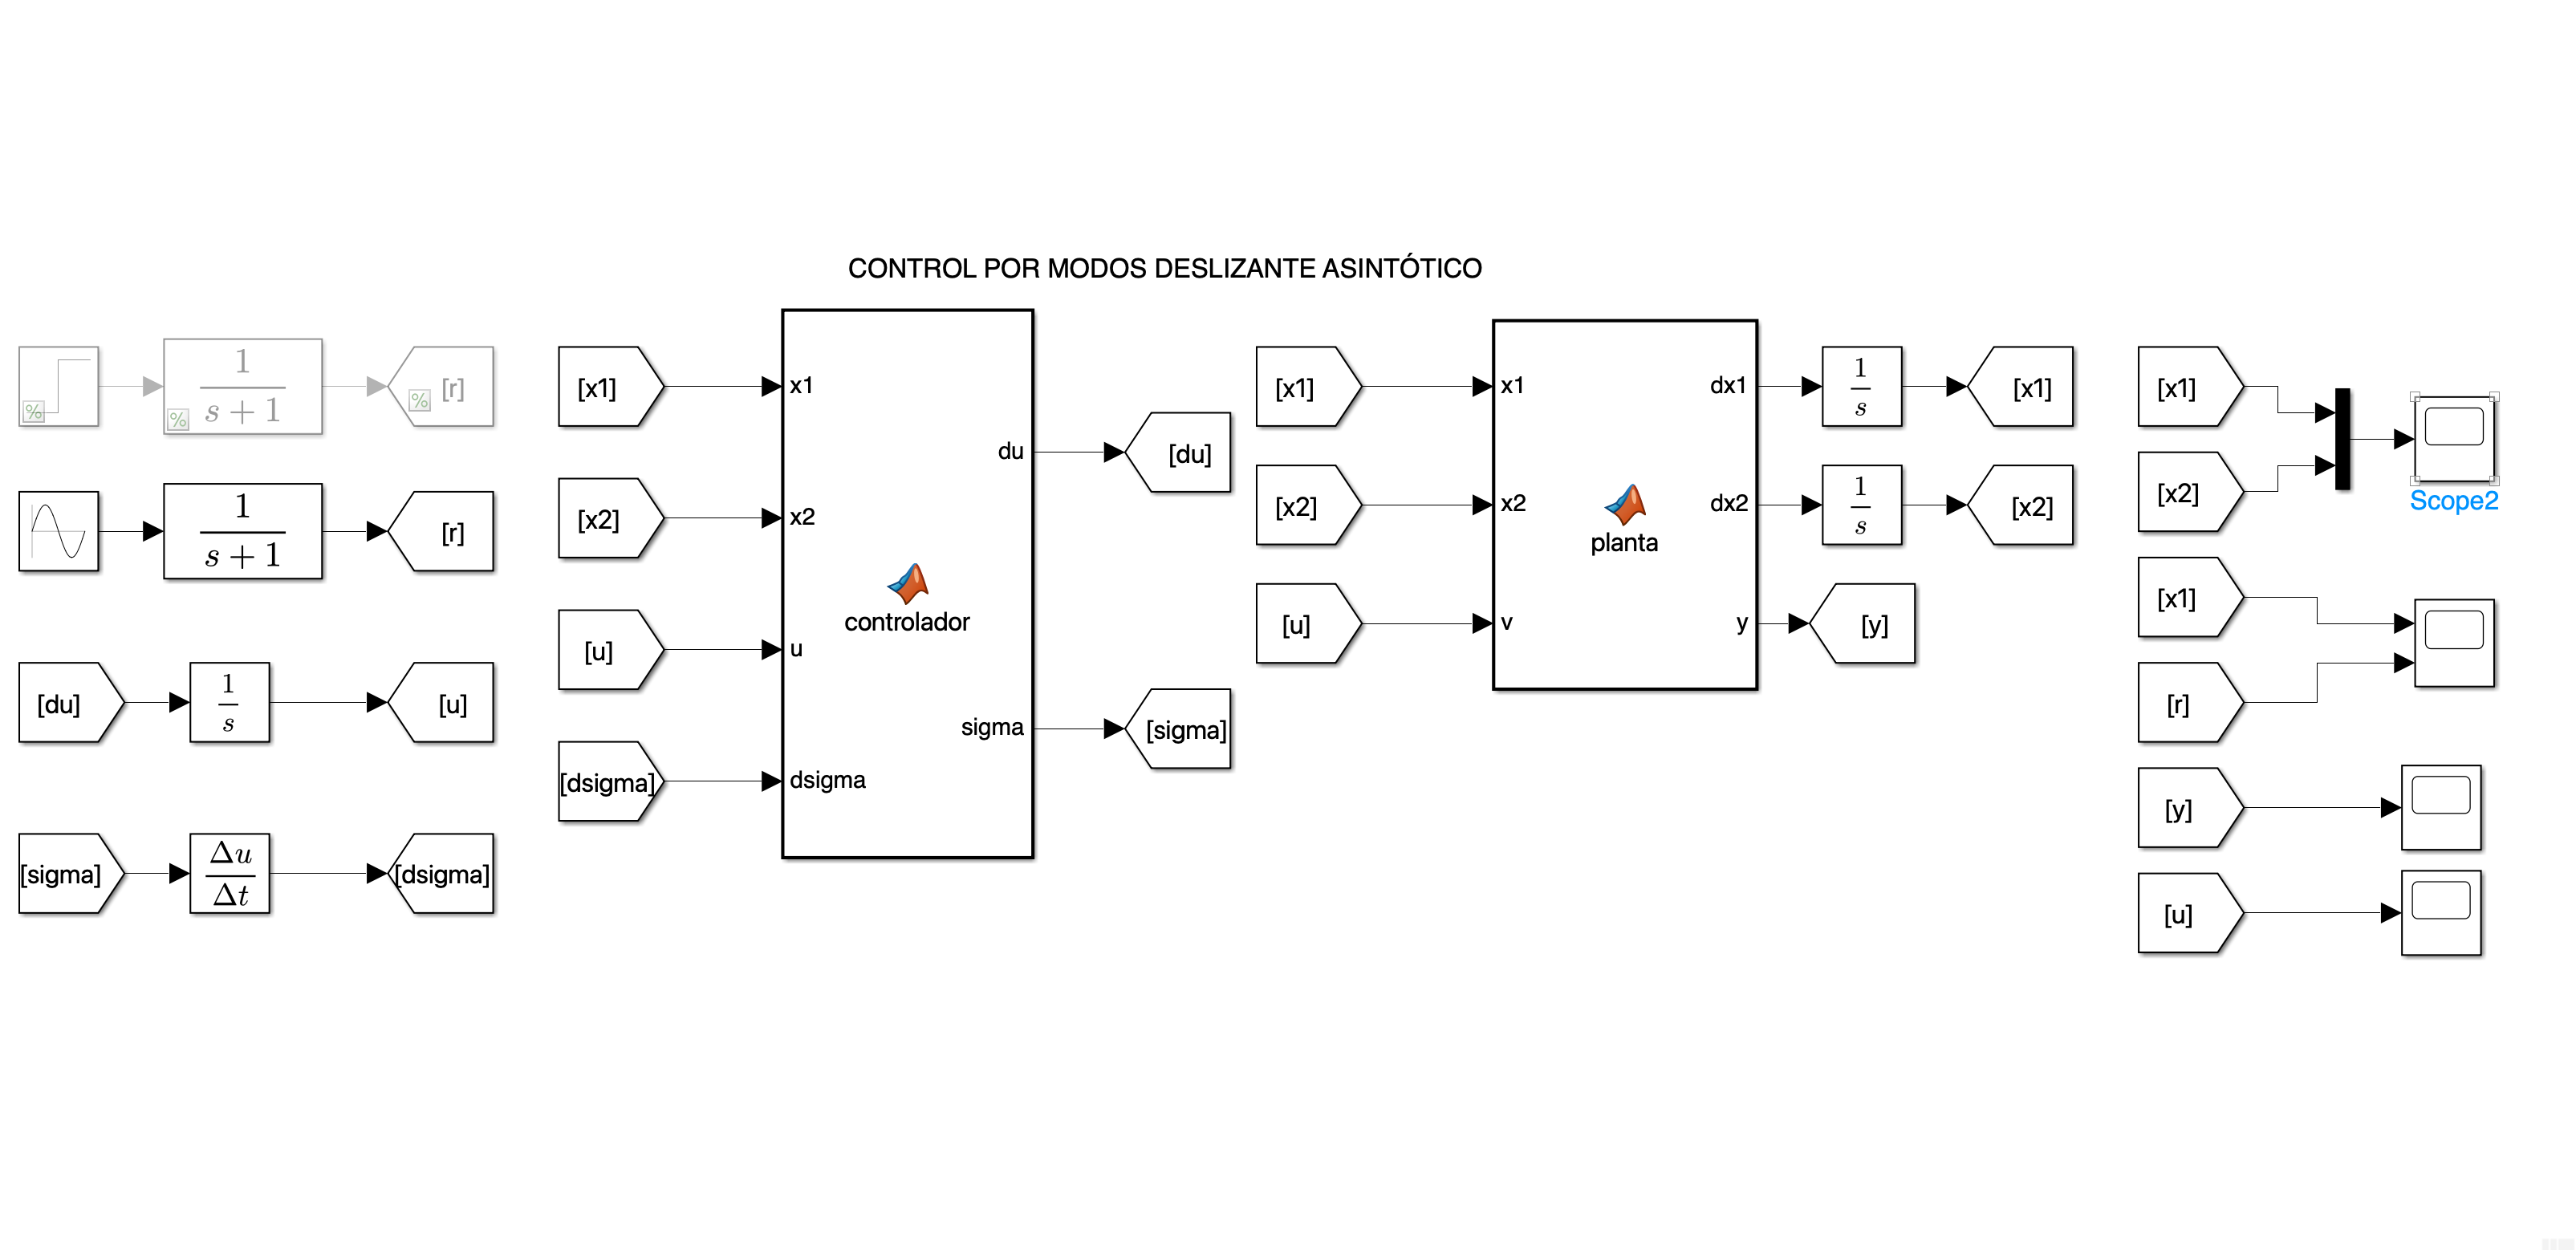
\includegraphics[width=0.8\textwidth]{img/SMC_asintotico.png}%
  }

  \small\textit{Haga clic en la imagen para abrir la carpeta de los modelos de Simulink y abra el archivo \texttt{SMC\_asintotico.slx} para ejecutar la simulación.}
\end{center}


\clearpage

\paragraph{\tituloejemplo{Ejemplo *PENDIENTE*}}
Verifique el funcionamiento del controlador pero ahora con seguimiento de trayectorias
\[
  \dot{X}_1=X_2
\]
\[
  \dot{X}_2=\operatorname{sen}(X_1X_2)+\cos(X_1+X_2)+u
\]
\[
  y=X_1
\]

\paragraph{Resolución}

El controlador se implementa dentro de un bloque \texttt{MATLAB Function}:

\begin{MatlabCode}
function [du, sigma]= controlador(x1, e, u, dsigma)

% Ganancia K>1
K = 115;

% Valor arbitrario positivo
m = 4.57;
ms = 72;

sigma = e + m*x1;
s = dsigma + ms*sigma;
du = +m*ms*e - (m+ms)*u - K*sign(s);
\end{MatlabCode}

La planta también se implementa dentro de un bloque
\texttt{MATLAB Function}:

\begin{MatlabCode}
function [dx1, dx2, y] = planta(x1, x2, v)

dx1 = x2;
dx2 = sin(x1+x2) + cos(x1*x2) + v;
y = x1;
\end{MatlabCode}

\begin{center}
  \href{file:../../sim/Parcial\%201/}{%
    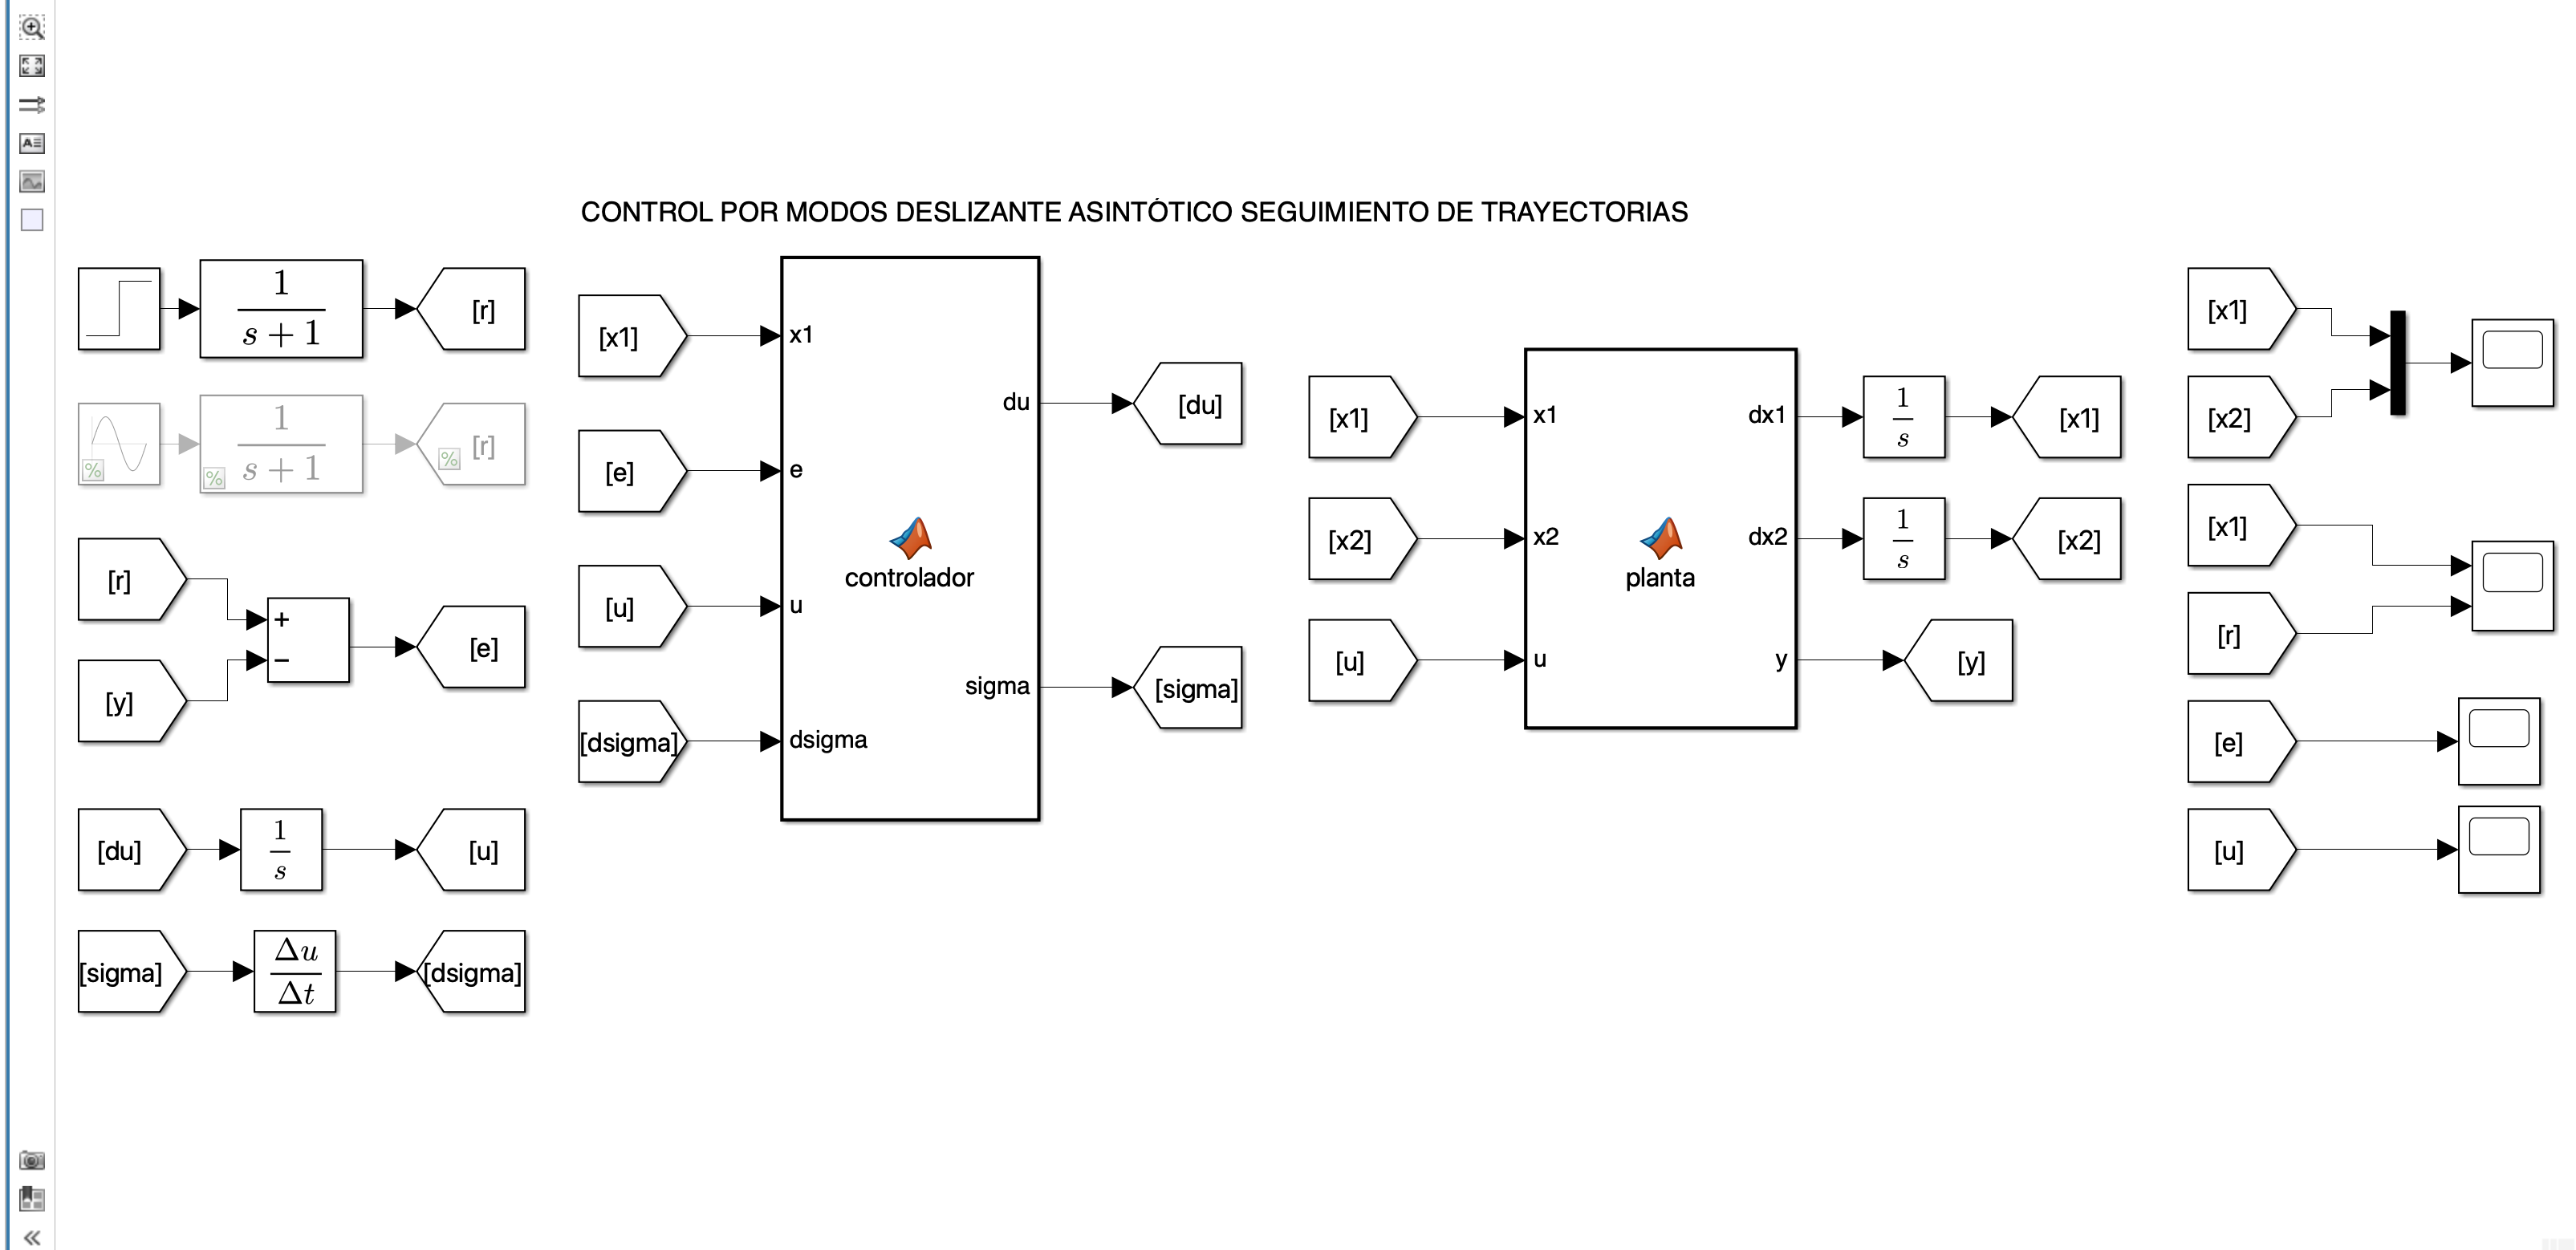
\includegraphics[width=0.8\textwidth]{img/SMC_asintotico_seg_tray.png}%
  }

  \small\textit{Haga clic en la imagen para abrir la carpeta de los modelos de Simulink y abra el archivo \texttt{SMC\_asintotico\_seg\_tray.slx} para ejecutar la simulación.}
\end{center}
